\documentclass[tikz,border=4pt]{standalone}
\usepackage{amsmath,amssymb}
\usetikzlibrary{positioning,arrows.meta,calc,fit}
\begin{document}
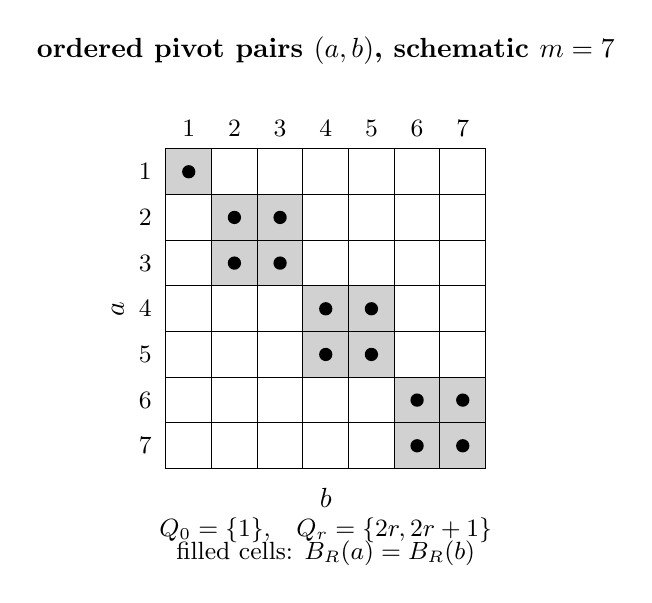
\begin{tikzpicture}[x=.58cm,y=.58cm,font=\small]
\node[font=\bfseries] at (4.5,1.15) {ordered pivot pairs $(a,b)$, schematic $m=7$};
\foreach \a in {1,...,7}{\foreach \b in {1,...,7}{\draw (\b,-\a) rectangle +(1,-1);}}
% Q0 singleton block.
\fill[black!18] (1,-1) rectangle +(1,-1);
\fill (1.5,-1.5) circle (2.4pt);
% Qr 2x2 blocks for r=1,2,3.
\foreach \p/\q in {2/3,4/5,6/7}{
  \fill[black!18] (\p,-\p) rectangle +(2,-2);
  \foreach \a in {\p,\q}{\foreach \b in {\p,\q}{\fill (\b+.5,-\a-.5) circle (2.4pt);}}
}
\foreach \a in {1,...,7}{\foreach \b in {1,...,7}{\draw (\b,-\a) rectangle +(1,-1);}}
\foreach \i in {1,...,7}{
  \node at (\i+.5,-.55) {$\i$};
  \node at (.55,-\i-.5) {$\i$};
}
\node[font=\bfseries] at (4.5,-8.65) {$b$};
\node[font=\bfseries,rotate=90] at (-.05,-4.5) {$a$};
\node[align=center] at (4.5,-9.35) {$Q_0=\{1\}$,\quad $Q_r=\{2r,2r+1\}$};
\node[align=center] at (4.5,-9.85) {filled cells: $B_R(a)=B_R(b)$};
\end{tikzpicture}
\end{document}
